\documentclass[aspectratio=169,11pt]{beamer}
\usetheme{Madrid}
\usepackage{tikz}
\usetikzlibrary{arrows.meta,positioning,calc}
\usepackage{amsmath,graphicx,booktabs}
\definecolor{navy}{HTML}{26384A}
\definecolor{blue}{HTML}{2980B9}
\definecolor{teal}{HTML}{168C82}
\definecolor{orange}{HTML}{DE8B35}
\definecolor{muted}{HTML}{64748B}
\definecolor{pale}{HTML}{F2F6FA}
\setbeamercolor{structure}{fg=blue}
\setbeamercolor{frametitle}{fg=white,bg=navy}
\setbeamercolor{normal text}{fg=navy,bg=white}
\setbeamercolor{block title}{fg=white,bg=blue}
\setbeamercolor{block body}{fg=navy,bg=pale}
\setbeamertemplate{navigation symbols}{}
\setbeamertemplate{footline}{\leavevmode\hbox{\begin{beamercolorbox}[wd=.9\paperwidth,ht=2.6ex,dp=1.2ex,leftskip=1em]{normal text}\color{muted}\scriptsize Yashashwi Singhania \quad | \quad Fed-batch feed optimization\end{beamercolorbox}\begin{beamercolorbox}[wd=.1\paperwidth,ht=2.6ex,dp=1.2ex,rightskip=1em plus1fil]{normal text}\color{muted}\scriptsize\insertframenumber/\inserttotalframenumber\end{beamercolorbox}}}
\setbeamerfont{frametitle}{size=\large,series=\bfseries}
\setbeamersize{text margin left=7mm,text margin right=7mm}
\title{Optimising Fed-Batch Feed Strategies}
\author{Yashashwi Singhania}
\date{September 2026}
\graphicspath{{figures/}{../VIth-sem/}}
\newcommand{\captionline}[1]{\vspace{1mm}\par{\scriptsize\color{muted}#1}}
\newcommand{\imageframe}[3]{\begin{frame}{#1}\centering\includegraphics[width=\textwidth,height=.77\textheight,keepaspectratio]{#2}\captionline{#3}\end{frame}}
\tikzset{card/.style={rounded corners=3pt,fill=pale,draw=blue!25,minimum height=1.2cm,text width=2.6cm,align=center,font=\small},flow/.style={-{Stealth[length=3mm]},line width=1.3pt,draw=blue}}
\begin{document}

\begin{frame}[plain]
\begin{columns}
\begin{column}{.13\textwidth}
\includegraphics[width=\linewidth]{iit_bhu_logo.png}\end{column}
\begin{column}{.8\textwidth}{\small\color{muted}IIT (BHU), Varanasi \quad | \quad UG Project II}\end{column}
\end{columns}
\vspace{3mm}
{\LARGE\bfseries Optimising Fed-Batch\\[2mm] Feed Strategies}\par
\vspace{3mm}{\large\color{blue}A recap, the procedure, and new results}\par
\vspace{3mm}
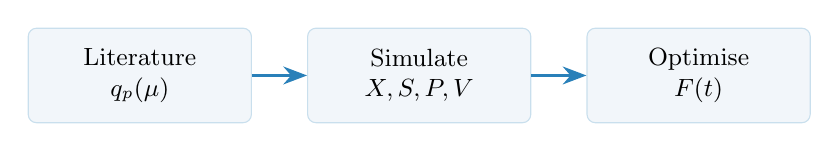
\begin{tikzpicture}
\node[card] (a) {Literature\\$q_p(\mu)$};
\node[card,right=7mm of a] (b) {Simulate\\$X,S,P,V$};
\node[card,right=7mm of b] (c) {Optimise\\$F(t)$};
\draw[flow] (a)--(b);\draw[flow] (b)--(c);
\end{tikzpicture}\par
\vspace{3mm}
{\small Yashashwi Singhania (23014019)\\Guide: Dr. Sharon Mano Pappu J.\\BPDD Laboratory, Biochemical Engineering}\par
\vspace{2mm}{\scriptsize\color{muted}September 2026 \quad | \quad July study, refreshed results}
\end{frame}

\begin{frame}{Recap 1: a browser interface for pyFOOMB}
\begin{columns}[c]
\begin{column}{.72\textwidth}
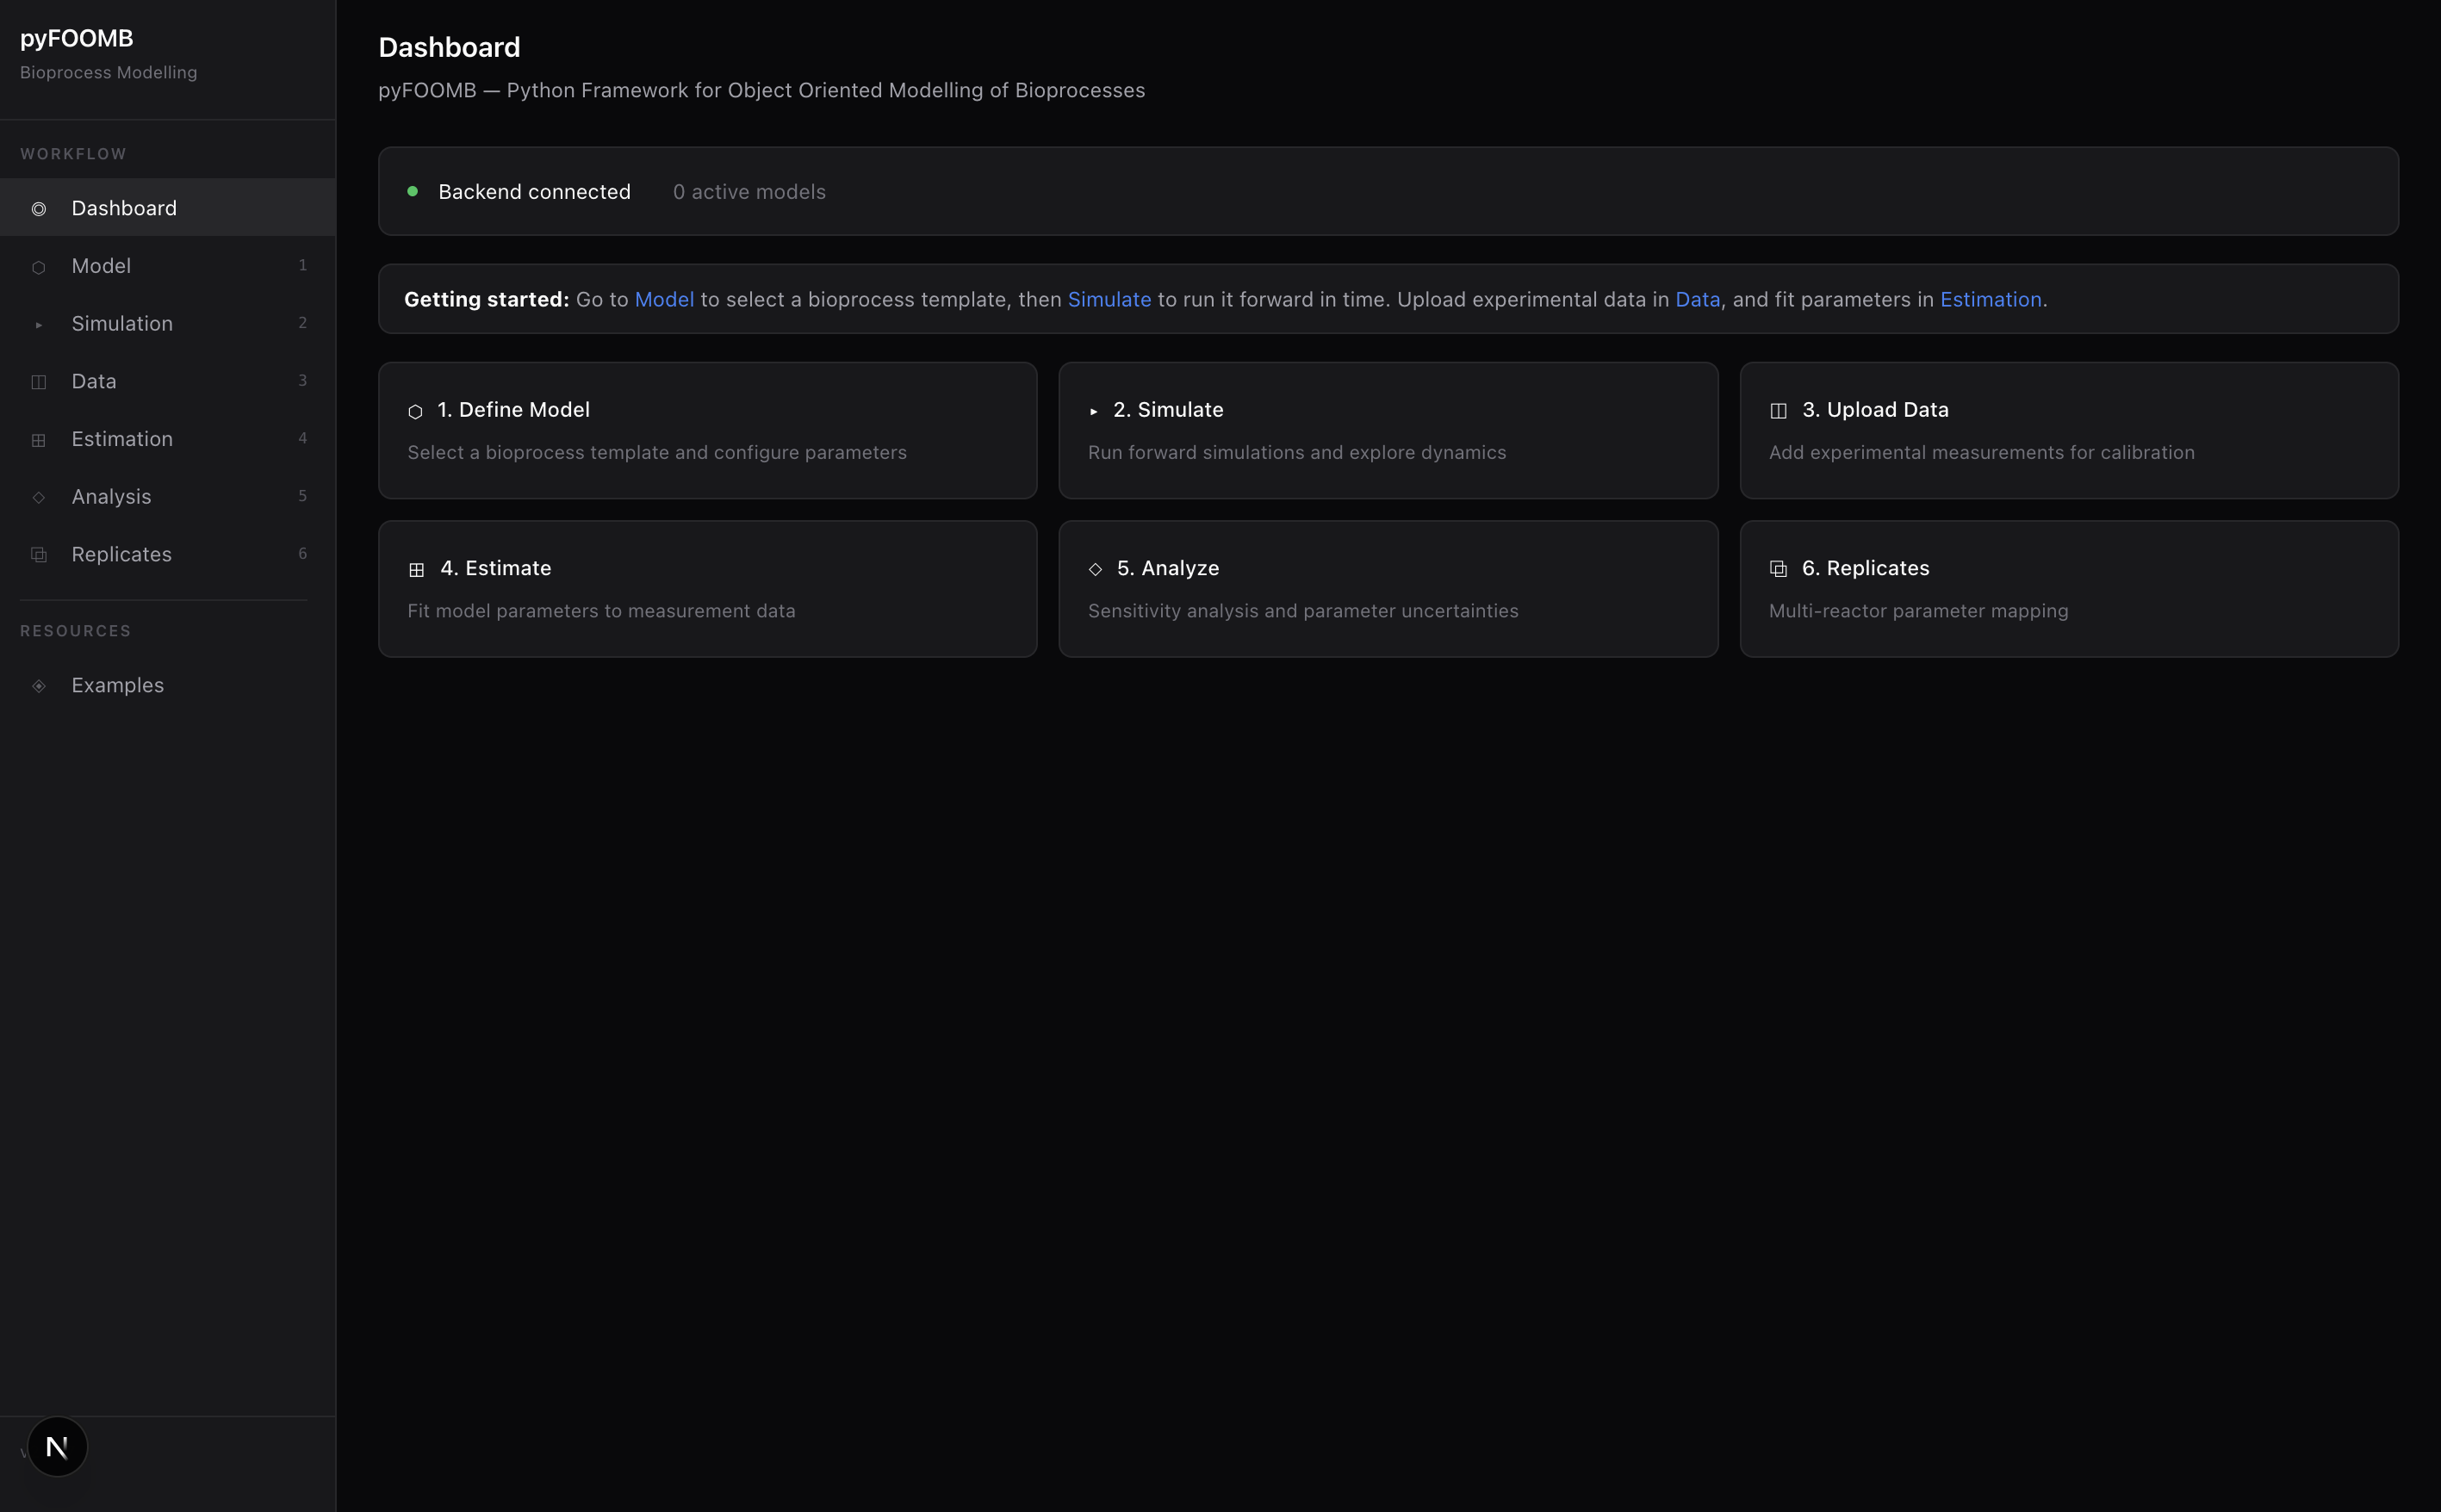
\includegraphics[trim=0 480bp 0 0,clip,width=\linewidth]{image.png}
\end{column}
\begin{column}{.25\textwidth}
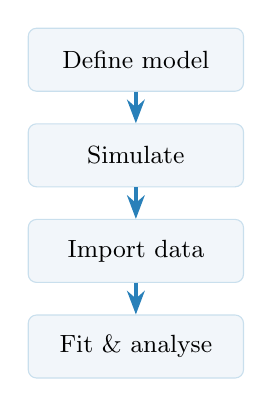
\begin{tikzpicture}[node distance=4mm]
\node[card,text width=2.5cm,minimum height=8mm] (a) {Define model};
\node[card,text width=2.5cm,minimum height=8mm,below=of a] (b) {Simulate};
\node[card,text width=2.5cm,minimum height=8mm,below=of b] (c) {Import data};
\node[card,text width=2.5cm,minimum height=8mm,below=of c] (d) {Fit \& analyse};
\draw[flow] (a)--(b);\draw[flow] (b)--(c);\draw[flow] (c)--(d);
\end{tikzpicture}
\end{column}
\end{columns}
\captionline{Actual interface from the VIth-semester work. Next.js frontend + FastAPI + pyFOOMB.}
\end{frame}

\imageframe{Recap 2: product formation depends on growth}{recap_qp_fits.png}{Representative literature fits from the 9-dataset study. Points: digitised data; lines: fitted models.}
\imageframe{Recap 3: turn fitted rates into batch profiles}{recap_batch.png}{Illustrative Fab 3H6 batch simulation. Generic Monod kinetics; this is a model prediction.}

\begin{frame}{New work: extend the model to fed-batch}
\begin{columns}[c]
\begin{column}{.55\textwidth}
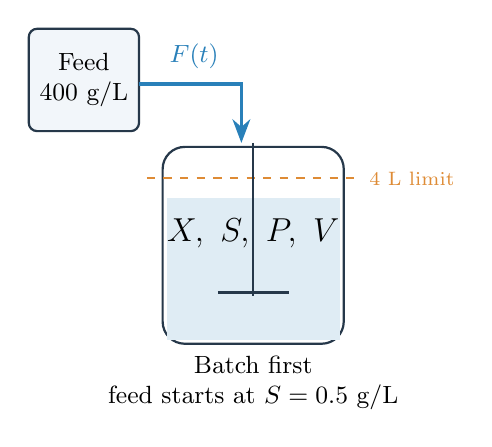
\begin{tikzpicture}[x=1cm,y=1cm]
\draw[thick,navy,rounded corners=3pt,fill=pale] (0,2.7) rectangle (1.4,4.0);
\node[font=\small,align=center] at (.7,3.35) {Feed\\400 g/L};
\draw[flow] (1.4,3.3)--(2.7,3.3)--(2.7,2.55);
\node[font=\small,blue] at (2.1,3.65) {$F(t)$};
\draw[thick,navy,rounded corners=8pt] (1.7,0) rectangle (4,2.5);
\fill[blue!15] (1.75,.05) rectangle (3.95,1.85);
\draw[dashed,orange,thick] (1.5,2.1)--(4.2,2.1);
\node[font=\scriptsize,orange,anchor=west] at (4.2,2.1) {4 L limit};
\draw[thick,navy] (2.85,2.55)--(2.85,.6);
\draw[thick,navy] (2.4,.65)--(3.3,.65);
\node[font=\large] at (2.85,1.4) {$X,\ S,\ P,\ V$};
\node[font=\small,align=center] at (2.85,-.5) {Batch first\\feed starts at $S=0.5$ g/L};
\end{tikzpicture}
\end{column}
\begin{column}{.42\textwidth}
{\large\color{blue}One shared reactor}\par\vspace{3mm}
\begin{align*}
\dot X&=\mu X-\frac{F}{V}X\\
\dot S&=\frac{F}{V}(S_{in}-S)-\frac{\mu}{Y_{X/S}}X\\
\dot P&=q_p(\mu)X-\frac{F}{V}P\\
\dot V&=F
\end{align*}
\vspace{2mm}{\small 40 h feed phase\quad |\quad 2 L/h pump cap}
\end{column}
\end{columns}
\captionline{Monod: $\mu=\mu_{max}S/(K_S+S)$. Feed changes substrate availability, which changes growth and production.}
\end{frame}

\imageframe{Seven feed patterns, one comparison}{feed_strategy_schematics.png}{Illustrative shapes. Each strategy's parameters are optimized separately for each of the 9 datasets.}

\begin{frame}{Analytical procedure: fit, simulate, optimise}
\vspace{2mm}
\begin{center}
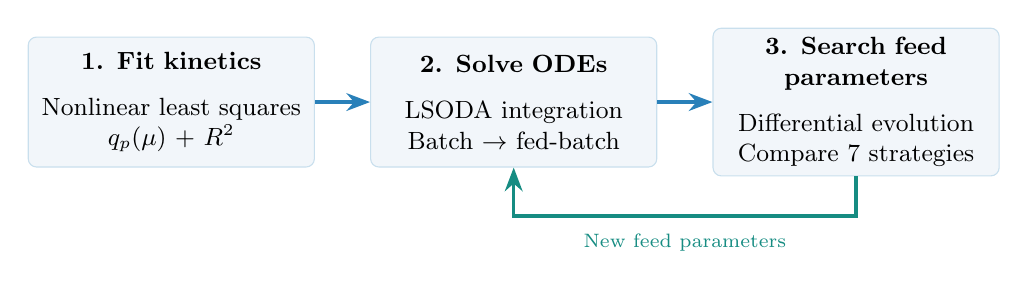
\begin{tikzpicture}[node distance=7mm]
\node[card,text width=3.4cm,minimum height=1.65cm] (fit) {\textbf{1. Fit kinetics}\\[2mm]Nonlinear least squares\\$q_p(\mu)$ + $R^2$};
\node[card,text width=3.4cm,minimum height=1.65cm,right=of fit] (sim) {\textbf{2. Solve ODEs}\\[2mm]LSODA integration\\Batch $\rightarrow$ fed-batch};
\node[card,text width=3.4cm,minimum height=1.65cm,right=of sim] (opt) {\textbf{3. Search feed parameters}\\[2mm]Differential evolution\\Compare 7 strategies};
\draw[flow] (fit)--(sim);\draw[flow] (sim)--(opt);
\draw[flow,teal] (opt.south)--++(0,-.5)-|(sim.south);
\node[font=\scriptsize,text=teal] at ($(sim.south)!0.5!(opt.south)+(0,-.9)$) {New feed parameters};
\end{tikzpicture}
\end{center}
\vspace{3mm}
\begin{columns}[c]
\begin{column}{.48\textwidth}
\begin{block}{Objective}\centering\Large Maximise $P(t_f)\,V(t_f)$\end{block}
\centering{\small Concentration $\times$ volume = total amount}
\end{column}
\begin{column}{.48\textwidth}
\centering{\large\color{blue}9 datasets $\times$ 7 strategies = 63 cases}\par
\vspace{3mm}{\small Propose feeds $\rightarrow$ simulate $\rightarrow$ score\\$\rightarrow$ evolve better candidates}
\end{column}
\end{columns}
\vspace{4mm}
\captionline{SciPy implementation. Seed 42; up to 40 DE generations; population multiplier 14. Rankings are indicative.}
\end{frame}

\imageframe{A necessary correction: stop feeding at 4 L}{volume_validation.png}{Before: a soft penalty allowed overflow. Now: the ODE stops the pump at the volume limit; all 63 candidate feeds verified with a terminal volume event.}

\imageframe{Which strategy performs well for each product?}{strategy_heatmap.png}{Each row is normalised to its own best result (100\%). Compare strategies within a product; units differ across products.}

\imageframe{One example: the optimised Fab 3H6 process}{fab_optimized_trajectory.png}{Feed, growth rate, and accumulated product from the corrected model. The dashed growth line marks the fitted $q_p$ peak.}

\begin{frame}{What the results tell us, and what comes next}
\vspace{2mm}
\begin{center}
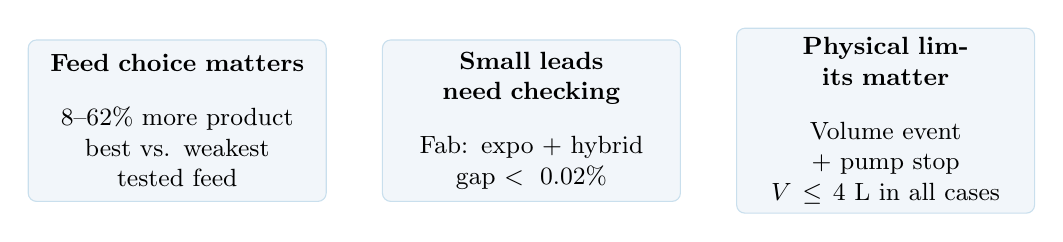
\begin{tikzpicture}[node distance=7mm]
\node[card,text width=3.55cm,minimum height=2.05cm] (a) {\textbf{Feed choice matters}\\[3mm]8--62\% more product\\best vs. weakest\\tested feed};
\node[card,text width=3.55cm,minimum height=2.05cm,right=of a] (b) {\textbf{Small leads need checking}\\[3mm]Fab: expo + hybrid\\gap $<0.02\%$};
\node[card,text width=3.55cm,minimum height=2.05cm,right=of b] (c) {\textbf{Physical limits matter}\\[3mm]Volume event + pump stop\\$V \leq 4$ L in all cases};
\end{tikzpicture}
\end{center}
\vspace{7mm}
\centering{\Large\color{blue}Next: verify robustness $\rightarrow$ validate with data $\rightarrow$ add to GUI}\par
\vspace{5mm}{\small Current scope: synthetic reactor assumptions and digitised literature kinetics.\\Repeat across seeds and test real fed-batch runs before choosing a lab feed.}\par
\vspace{5mm}{\small\color{muted}BPDD Laboratory \quad | \quad IIT (BHU), Varanasi}
\end{frame}
\end{document}
